\documentclass{article}
\usepackage[utf8]{inputenc}
\usepackage{geometry}
 \geometry{
 a4paper,
 total={170mm,257mm},
 left=20mm,
 top=20mm,
 }
\usepackage{polski}
\usepackage{natbib}
\usepackage[capbesideposition=right]{floatrow}
\usepackage{graphicx}
\usepackage{pbox}
\usepackage{float}
\usepackage[dvipsnames]{xcolor}
\usepackage{caption}
\usepackage{wrapfig}
\usepackage{graphicx}
\usepackage{tikz}
    \usetikzlibrary{
        arrows,
        shadows,
        shapes,
        automata,
        positioning,
        arrows.meta
    }
\usepackage{pgfplots}
\usepackage{tabularx}
\usepackage{booktabs}
\usepackage{amsfonts}
\pgfplotsset{compat=1.17}

\begin{document}
\centering 
\Huge State Machine Diagram
\vspace{1cm}
\normalsize
    
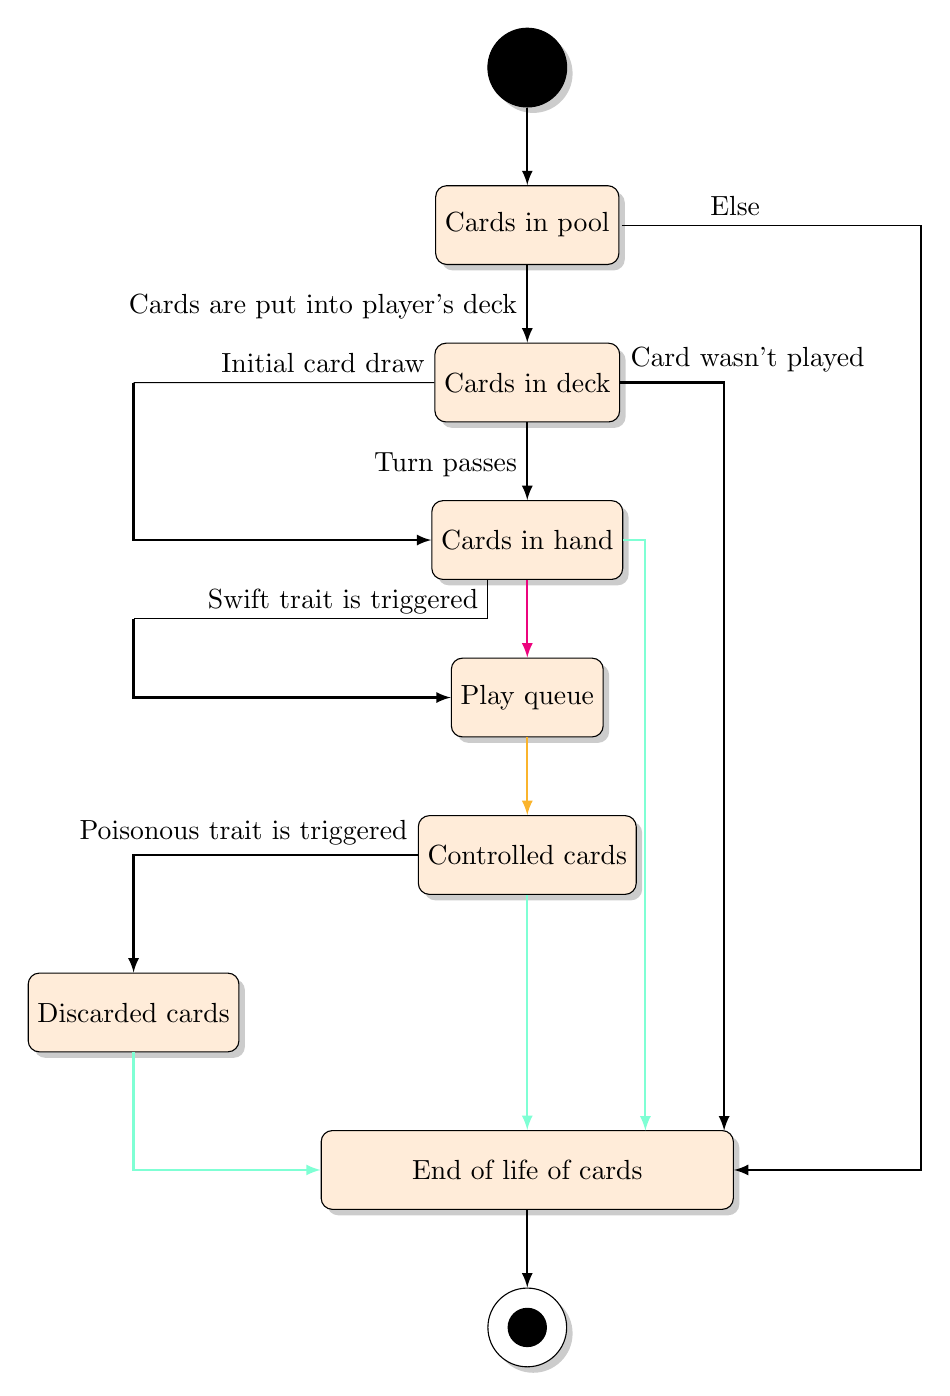
\begin{tikzpicture}
[baseshape/.style={minimum width=1cm, minimum height=1cm,text centered, font=\normalsize,draw=black, drop shadow=black!40},
startstop/.style={baseshape, circle, fill=black},
stop/.style={circle, fill =black},
io/.style={baseshape, trapezium, trapezium stretches=true, 
trapezium left angle=70, trapezium right angle=110, fill=blue!30},
process/.style={baseshape, rectangle, rounded corners, fill=orange!15},
decision/.style={baseshape, diamond, minimum width=1cm, fill=white},
block/.style={baseshape, rectangle, minimum width=1cm, fill=white},
arrow/.style={thick, -latex},
node distance=2cm,]
\node (start) [startstop]{};
\node (step1) [process, below of=start]{Cards in pool};
\node (step2) [process, below of=step1]{Cards in deck};
\node (step3) [process, below of=step2]{Cards in hand};
\node (step4) [process, below of=step3]{Play queue};
\node (step5) [process, below of=step4]{Controlled cards};
\node (step6) [process, below of=step5, xshift = -5cm]{Discarded cards};
\node (step7) [process, below of=step6, xshift = 5cm, text width = 5cm]{End of life of cards};
\node (stop) [startstop, fill = white, below of=step7]{};
\node (stopka) [stop, minimum width  = 0.5cm, minimum height=0.5cm, below of=step7]{};

\draw [arrow] (start) -- (step1);
\draw [arrow] (step1) -- node[near start, anchor= north east]{Cards are put into player's deck}(step2);
\draw [arrow] (step2) -- node[near start, anchor= north east]{Turn passes}(step3);
\draw [arrow, RubineRed] (step3) -- (step4);
\draw [arrow, Dandelion] (step4) -- (step5);
\draw [arrow] (step5) -| node[at start, anchor = south east]{Poisonous trait is triggered}(step6);
\draw [arrow, Aquamarine] (step5) -- (step7);
\draw [arrow, Aquamarine] (step6) |- (step7);
\draw [arrow] (step7) -- (stop);

\draw (step2) -- node[at start, anchor= south east]{Initial card draw}(-5, -4);
\draw [arrow] (-5, -4) |- (step3);

\draw (1.2, -2) -- node[at start, anchor= south west, xshift =1cm]{Else}(5, -2);
\draw [arrow] (5, -2) |- (step7);

\draw [arrow] (step2) -| node[at start, anchor= south west]{Card wasn't played}(2.5, -13.5);

\draw [arrow, Aquamarine] (step3) -| node[at start, anchor= south, color = Aquamarine, yshift =0.5cm, xshift = 0.1cm]{}(1.5, -13.5);

\draw (-0.5, -6.5) |- node[at start, anchor = north east]{Swift trait is triggered}(-5, -7);
\draw [arrow] (-5, -7) |- (step4);


\end{tikzpicture}
\\
\begin{flushleft}
\textcolor{Aquamarine}{Game ends} \\
\textcolor{RubineRed}{Card is selected by the player} \\
\textcolor{Dandelion}{Card is put onto the table}
\end{flushleft}
\end{document}